\documentclass[xcolor=dvipsnames]{beamer}

\usetheme{Madrid}

\usecolortheme{whale}

\useoutertheme[]{sidebar}

\setbeamercovered{transparent}


\usepackage[english]{babel}
\usepackage[T1]{fontenc}
\usepackage[utf8]{inputenc}
\usepackage{url}
\usepackage{tikz}
\usepackage{graphicx}

\usepackage{listings}
\usepackage[scaled]{uarial}
\renewcommand*\familydefault{\sfdefault}
\usepackage[T1]{fontenc}


%\lstset{language=C++,basicstyle=\fontsize{8}{9.6}\selectfont,showstringspaces=false,columns=fullflexible,identifierstyle=\ttfamily,keywordstyle=\bfseries,showstringspaces=false,columns=fullflexible}
\lstset{language=C,basicstyle=\fontsize{10}{13}\selectfont,identifierstyle=\ttfamily,keywordstyle=\bfseries,showstringspaces=false,columns=fixed}

\def\BibTeX{\textsc{Bib}\kern-.08em\TeX} 

\newcommand{\footcite}[1]{\footnote{\tiny #1}}
\newcommand{\umlet}{.5}
\newcommand{\emp}[1]{\textit{\alert{#1}}}
\newcommand{\kw}[1]{\mbox{\textbf{#1}}}
\newcommand{\id}[1]{\texttt{#1}}
\newcommand{\stl}{\guillemotleft}
\newcommand{\str}{\guillemotright}

\newcommand{\lsti}{\lstinline[basicstyle=\fontsize{10.5}{12.1}\selectfont]}

\newcommand{\ssection}[1]{
	\section{#1}
	\begin{frame}[fragile=singleslide]\frametitle{}
	\Huge #1
	\end{frame}
}

\newcommand{\ssectionn}[1]{
	\section*{#1}
	\begin{frame}[fragile=singleslide]\frametitle{}
	\Huge #1
	\end{frame}
}

\newenvironment{program}{\begin{beamercolorbox}[rounded=true,shadow=true]{block body}\vspace{-3mm}}{\vspace{-2mm}\end{beamercolorbox}}

\setbeamercolor{fvystup}{fg=white,bg=white}
\newenvironment{vystup}{\begin{beamercolorbox}[rounded=true,shadow=true]{fvystup}}{\end{beamercolorbox}}

\newenvironment{poznamka}{\begin{beamercolorbox}[rounded=true,shadow=false]{block body}}{\end{beamercolorbox}}

\setbeamertemplate{footline}[page number]
{
%\insertpagenumber
%\begin{beamercolorbox}{section in head/foot}
%\vskip2pt\insertnavigation{\paperwidth}\vskip2pt
%\end{beamercolorbox}%
}

\setbeamercolor{frametitle}{fg=white}

\author{Maksim Alehash}
%\url{www.fiit.stuba.sk/~vranic}, \url{vranic@fiit.stuba.sk}}
%{\tiny \url{www.fiit.stuba.sk/~vranic}, \url{vranic@fiit.stuba.sk}}
\institute{
	Ústav informatiky, informačných systémov a softvérového inžinierstva\\
	Fakulta informatiky a informačných technológií\\
	Slovenská technická univerzita v Bratislave}

\subtitle{\vspace{5mm} Metódy inžinierskej práce 2023/2024}

\title{\textbf{Real-time data processing in autonomous vehicles}}

\date{\footnotesize\today}

\logo{
\begin{tikzpicture}
\filldraw[fill=white, very thick]circle (.55);
\node at (0,0){
\includegraphics[width=1.3cm]{STU-FIIT.png}};
\end{tikzpicture}
}


\begin{document}

\begin{frame}[fragile=singleslide]
\titlepage
\end{frame}

%------------------------------------------------------------------------------------------------------------------------------

\section*{Introduction}

\begin{frame}[fragile=singleslide]\frametitle{\bf{Introduction}}


\begin{poznamka}
{\textbf{What is an autonomous vehicle?}}
\end{poznamka}
\begin{itemize}
\item A self-driving car that uses necessary hardware and AI algorithms to navigate without any human intervention
\end{itemize}

\begin{poznamka}
{\textbf{Why is data processing so important in it?}}
\end{poznamka}
         \begin{itemize}
	\item {\bf{Safety and comfort}} 
	\item {\bf{Navigation}} 
	\item {\bf{Maintenance}} 
	\item {\bf{Effiency and effectivity}}
         \item {\bf{Machine learning}} 
	\item {\bf{Autonomy}}
	\end{itemize}

\end{frame}

%------------------------------------------------------------------------------------------------------------------------------

\begin{frame}[allowframebreaks]
\frametitle{\bf{Table of contents}}
\tableofcontents
\end{frame}


%------------------------------------------------------------------------------------------------------------------------------

\section{Sensors}

\begin{frame}[fragile=singleslide]\frametitle{\bf{Sensors}}
\centering
    \begin{figure}
    \centering
    \vspace*{-.1cm}
    \caption{Sensor coverage in AV\footnotemark}
    \footnotetext[1]{\tiny{\url{https://www.researchgate.net/figure/Sensors-coverage-diagram-for-an-autonomous-vehicle-taken-from-6_fig1_351407935/}}}
    \vspace*{-.3cm} 
    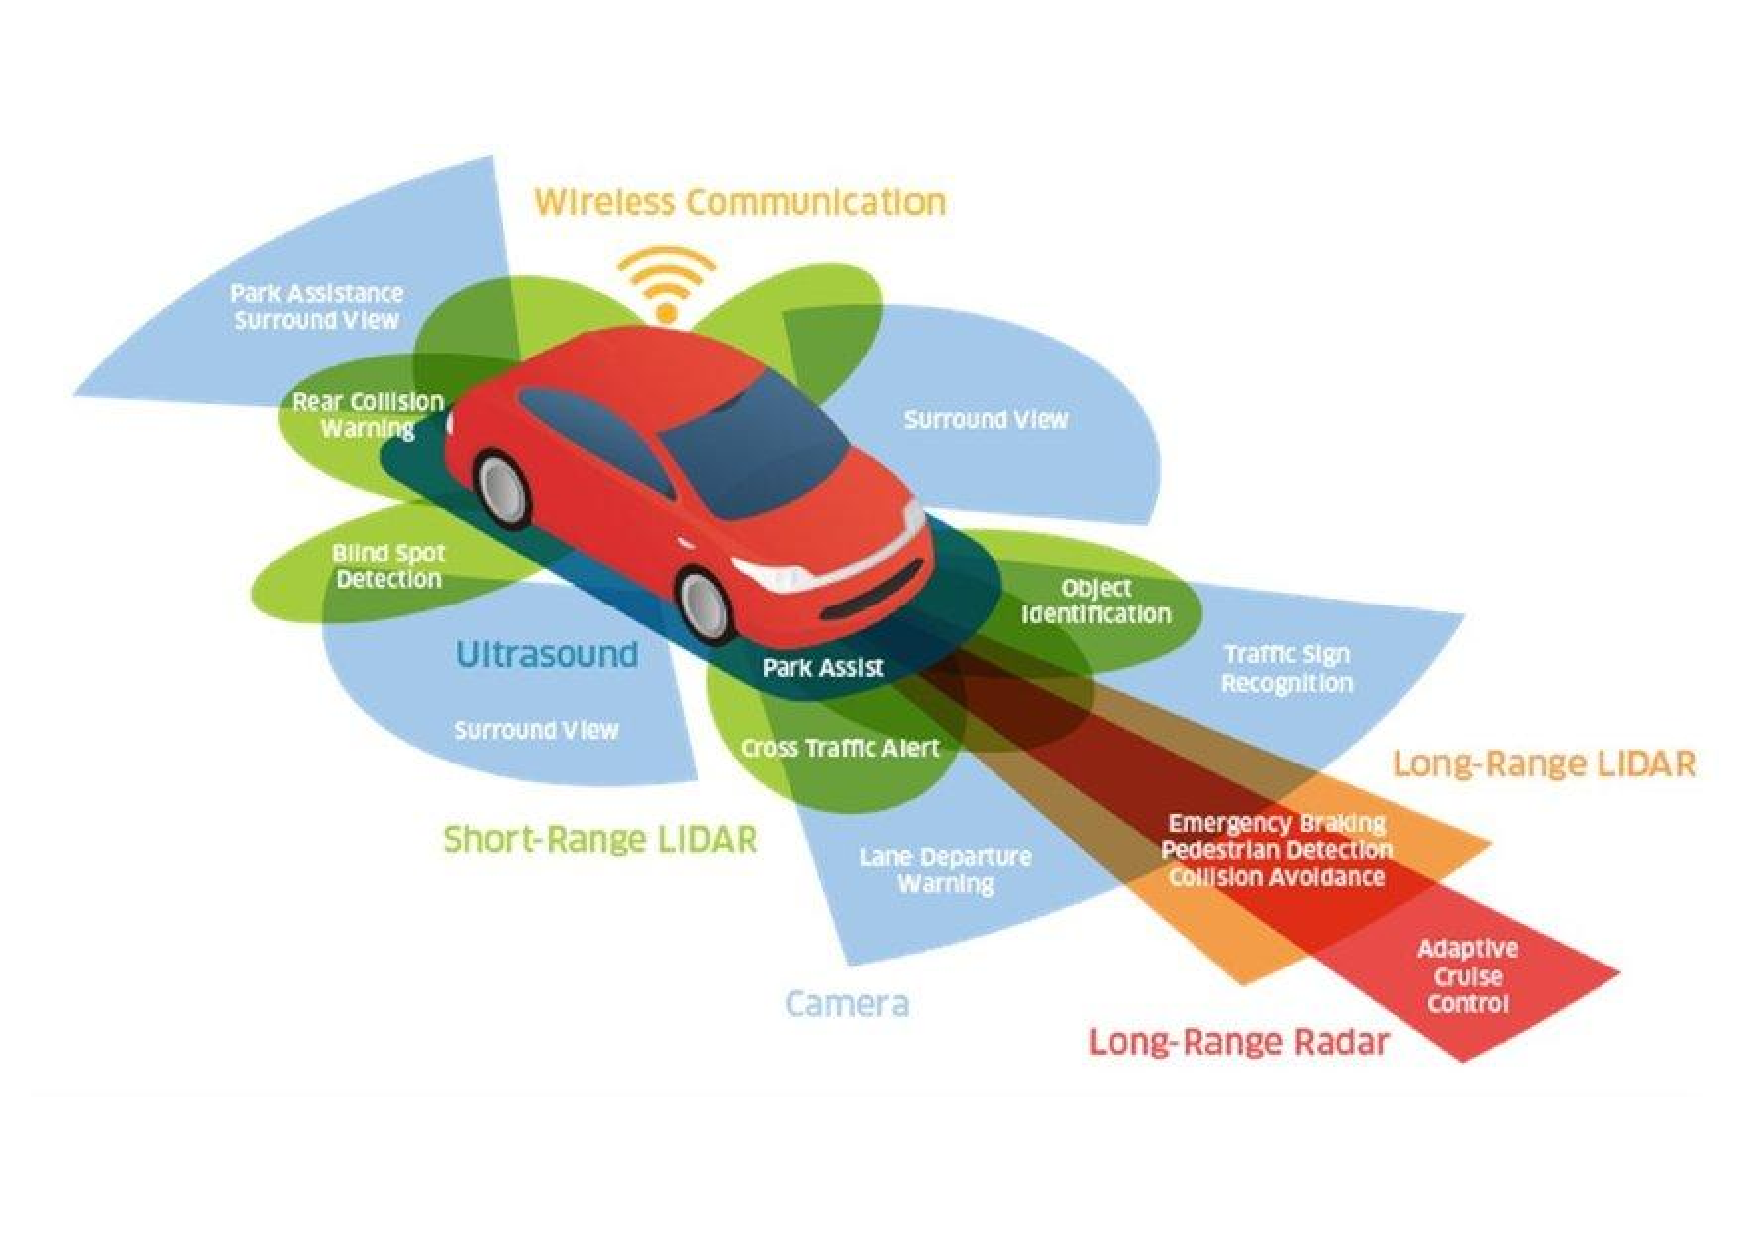
\includegraphics[width=9cm]{SensorsScheme.pdf}
    \end{figure}
\end{frame}

%------------------------------------------------------------------------------------------------------------------------------

\begin{frame}[fragile=singleslide]\frametitle{\bf{Sensors}}
\centering
    \begin{figure}
    \centering
    \caption{Advantages and disadvantages of sensors}
    \vspace*{-1.3cm}
    \hspace*{0.65cm}
    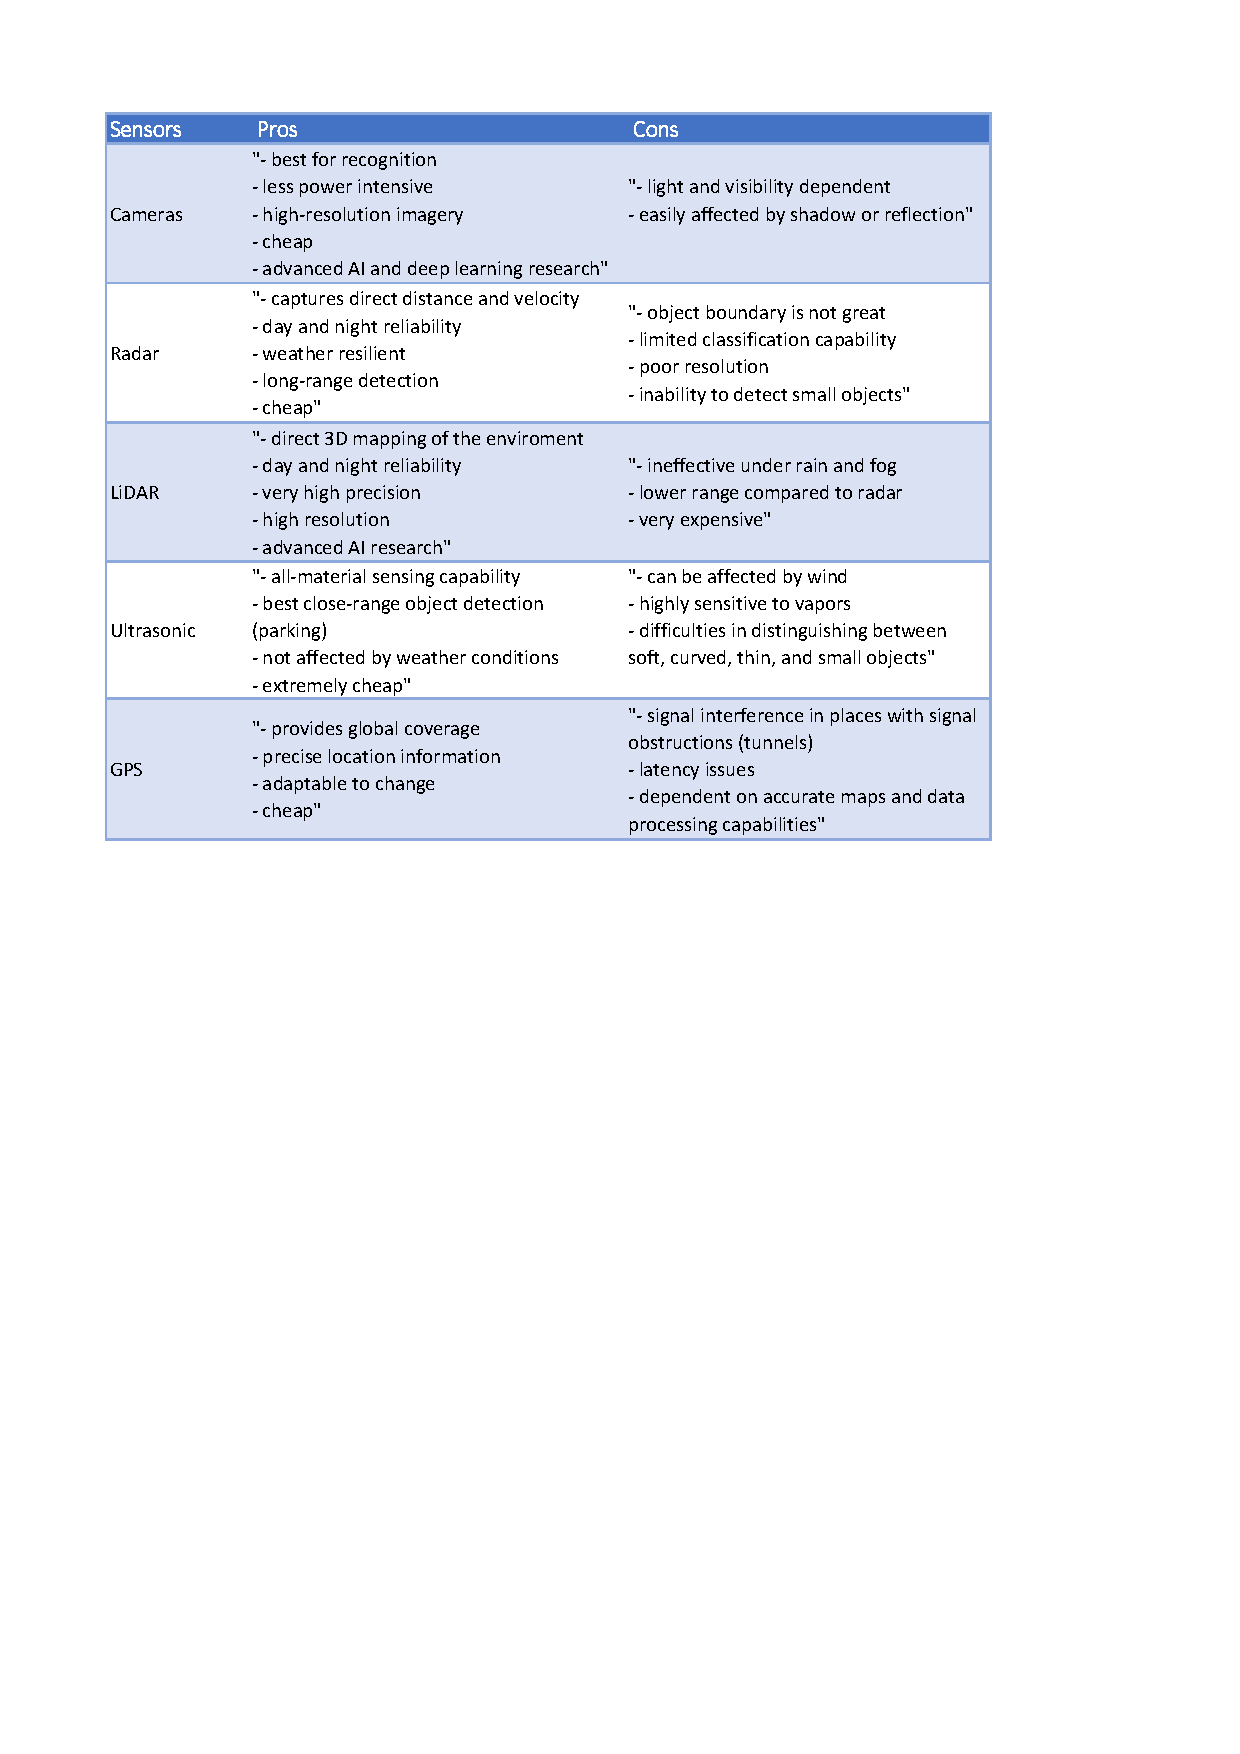
\includegraphics[width=10cm]{tabulka.pdf}
    \end{figure}
\end{frame}

%------------------------------------------------------------------------------------------------------------------------------

\section{Algorithms}

\begin{frame}[fragile=singleslide]\frametitle{\bf{Algorithms}}

\begin{block}{\textbf{AV divides data processing into 4 stages:}}
         \begin{itemize}
	\item {\bf{Mapping}} - creating a detailed representation of the enviroment
	\item {\bf{Localization}} - determining the precise position of the vehicle
	\item {\bf{Object detection}} - identyfing objects 
	\item {\bf{Object tracking}} - monitoring objects
	\item {\bf{Decision-making}} - utilizing processed data to make adaptive decisions
	\end{itemize}
\end{block}
\end{frame}

%------------------------------------------------------------------------------------------------------------------------------

\begin{frame}[fragile=singleslide]\frametitle{\bf{Algorithms}}
\centering
    \begin{figure}
    \centering
    \caption{Data acquisition and processing scheme}
    \vspace*{-.2cm}
    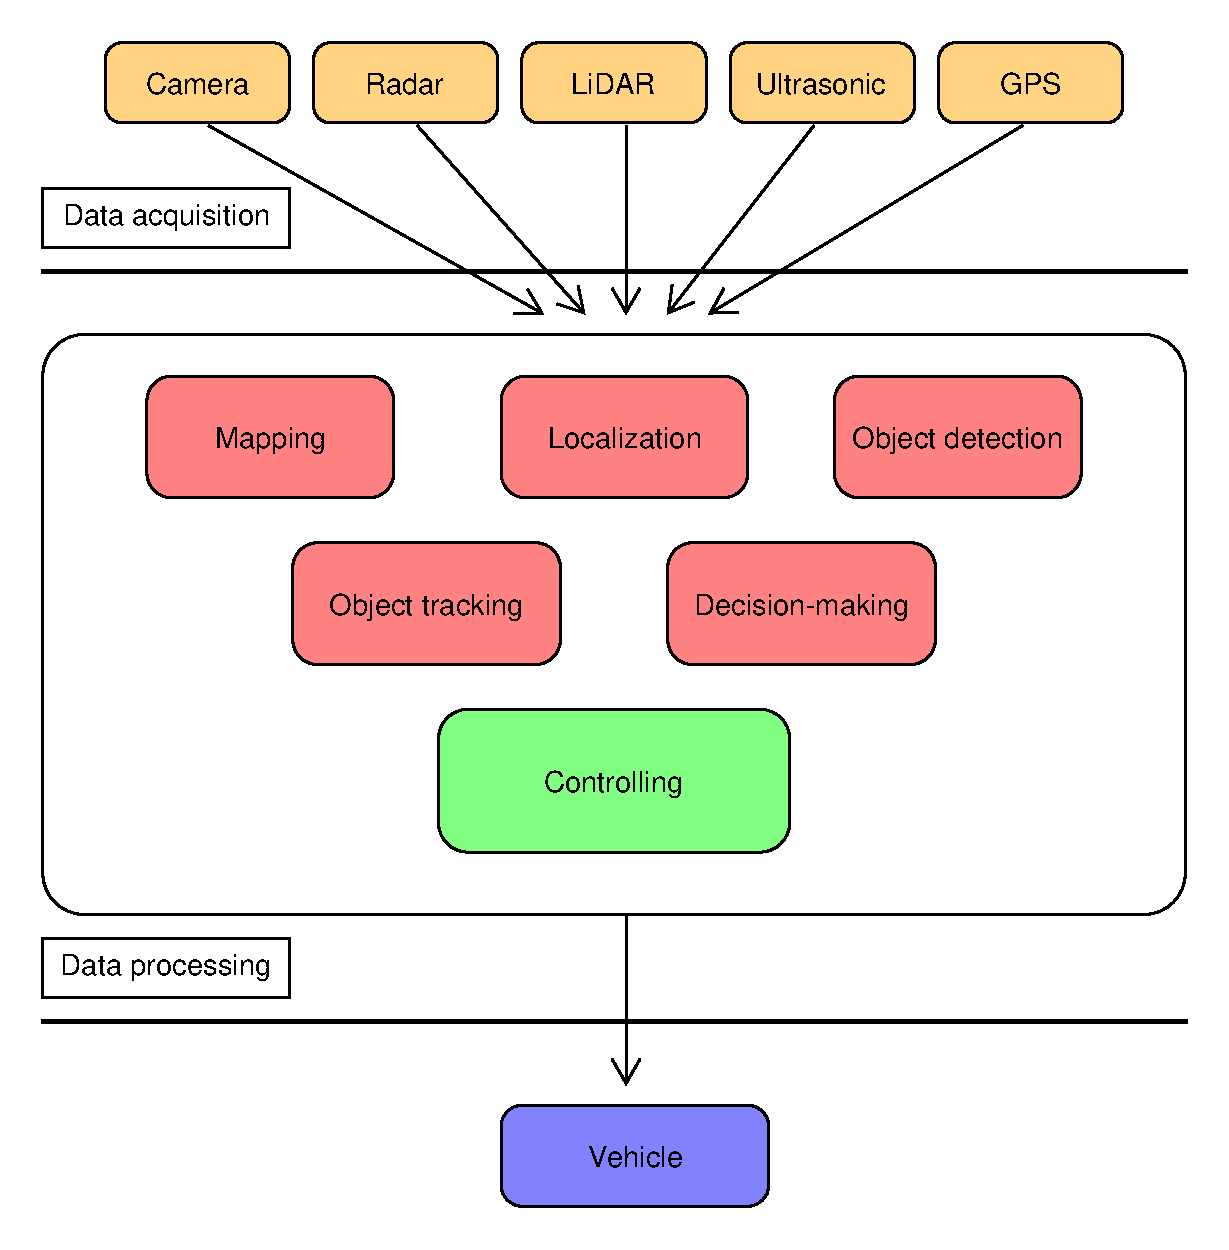
\includegraphics[width=6cm]{algoritmy.pdf}
    \end{figure}
\end{frame}

%------------------------------------------------------------------------------------------------------------------------------

\section{Data processing architecture}

\begin{frame}[fragile=singleslide]\frametitle{\bf{Data processing architecture}} 
\centering
    \begin{figure}
    \centering
    \caption{Mobile edge computing and vehicle communication\footnotemark}
    \footnotetext[2]{\tiny{\url{https://www.telematicswire.net/connected-vehicles-and-mobile-edge-computing-a-marriage-of-convenience/}}}
    \vspace*{-1.85cm}
    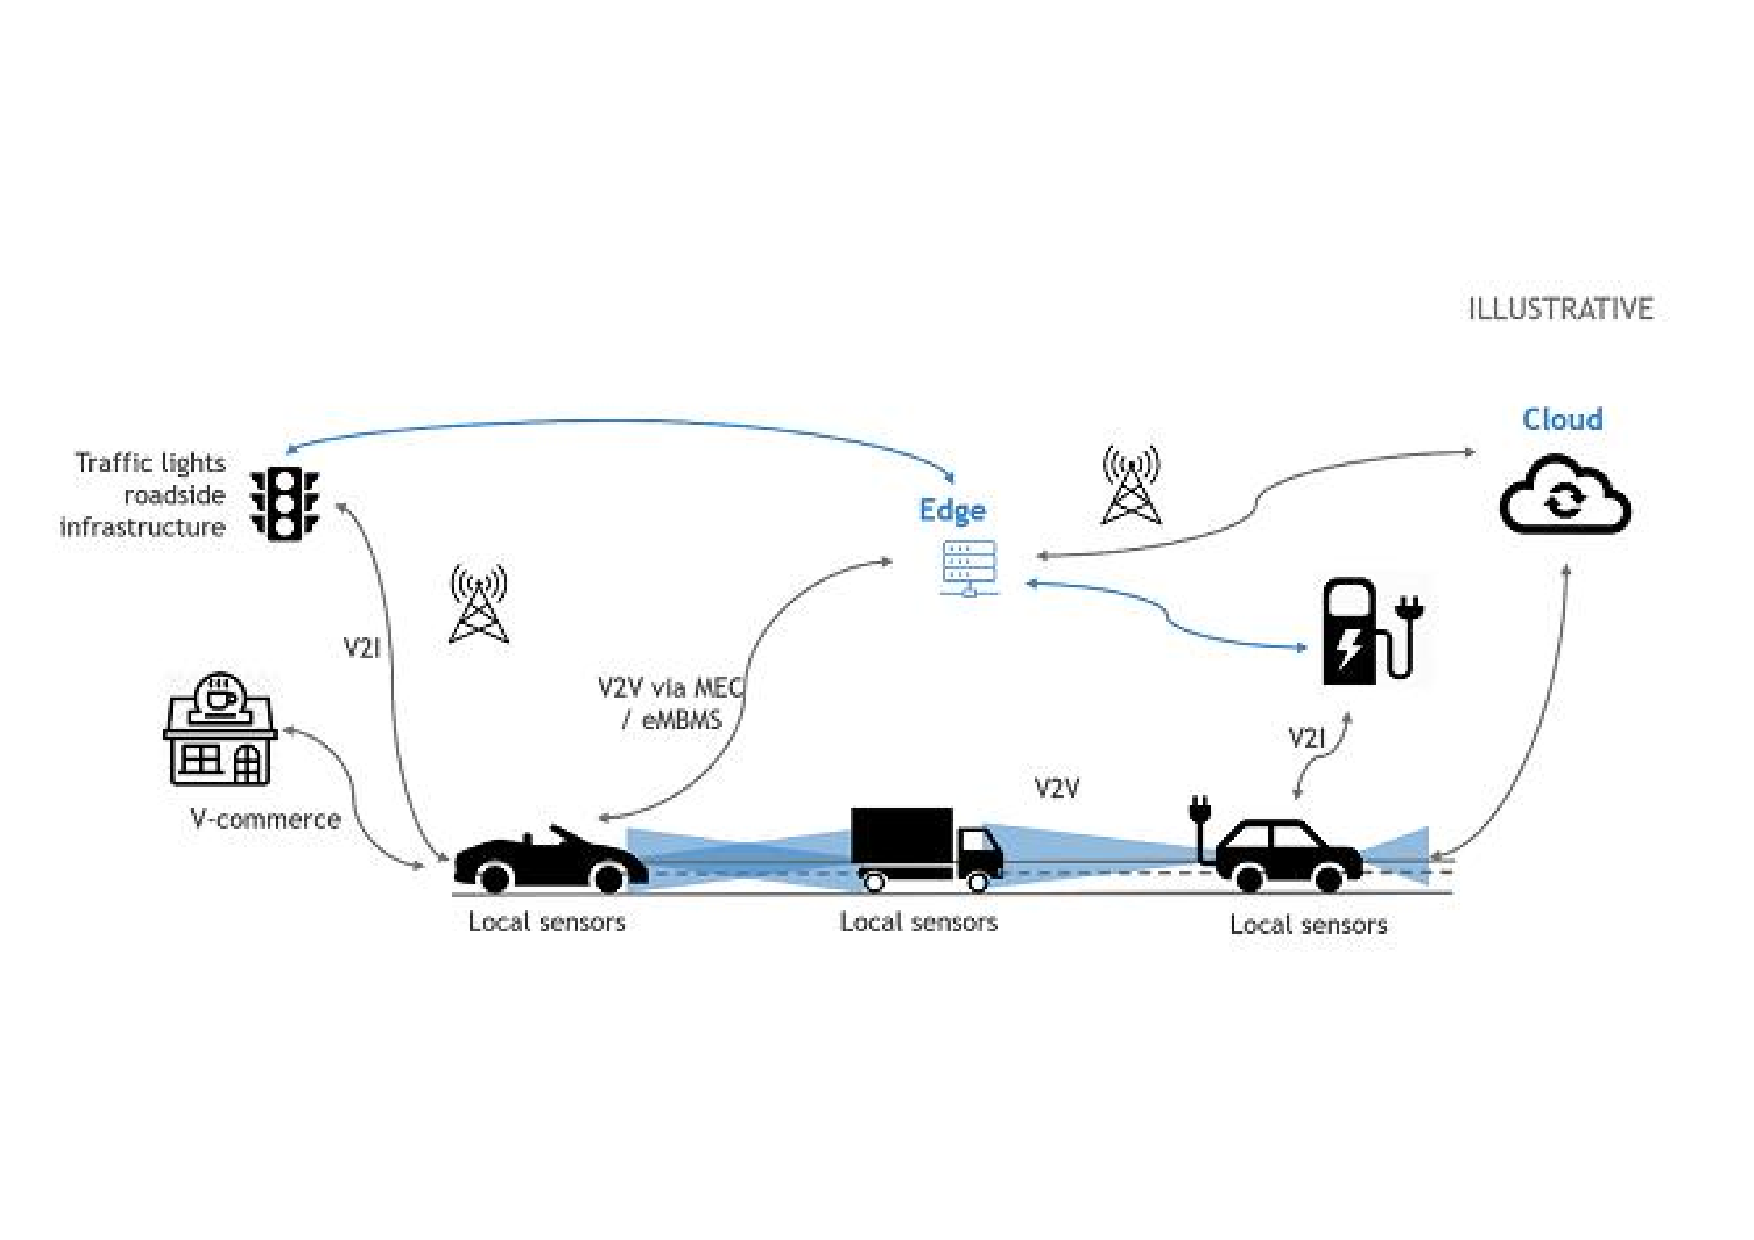
\includegraphics[width=10.5cm]{Edgecomputing.pdf}
    \end{figure}

\end{frame}

%------------------------------------------------------------------------------------------------------------------------------

\section{Safety challenges}

\begin{frame}[fragile=singleslide]\frametitle{\bf{Safety challenge}}
\centering
    \begin{figure}
    \vspace*{-.5cm}
    \caption{Challenges facing the safety of an AV}
    \hspace*{-.5cm}
    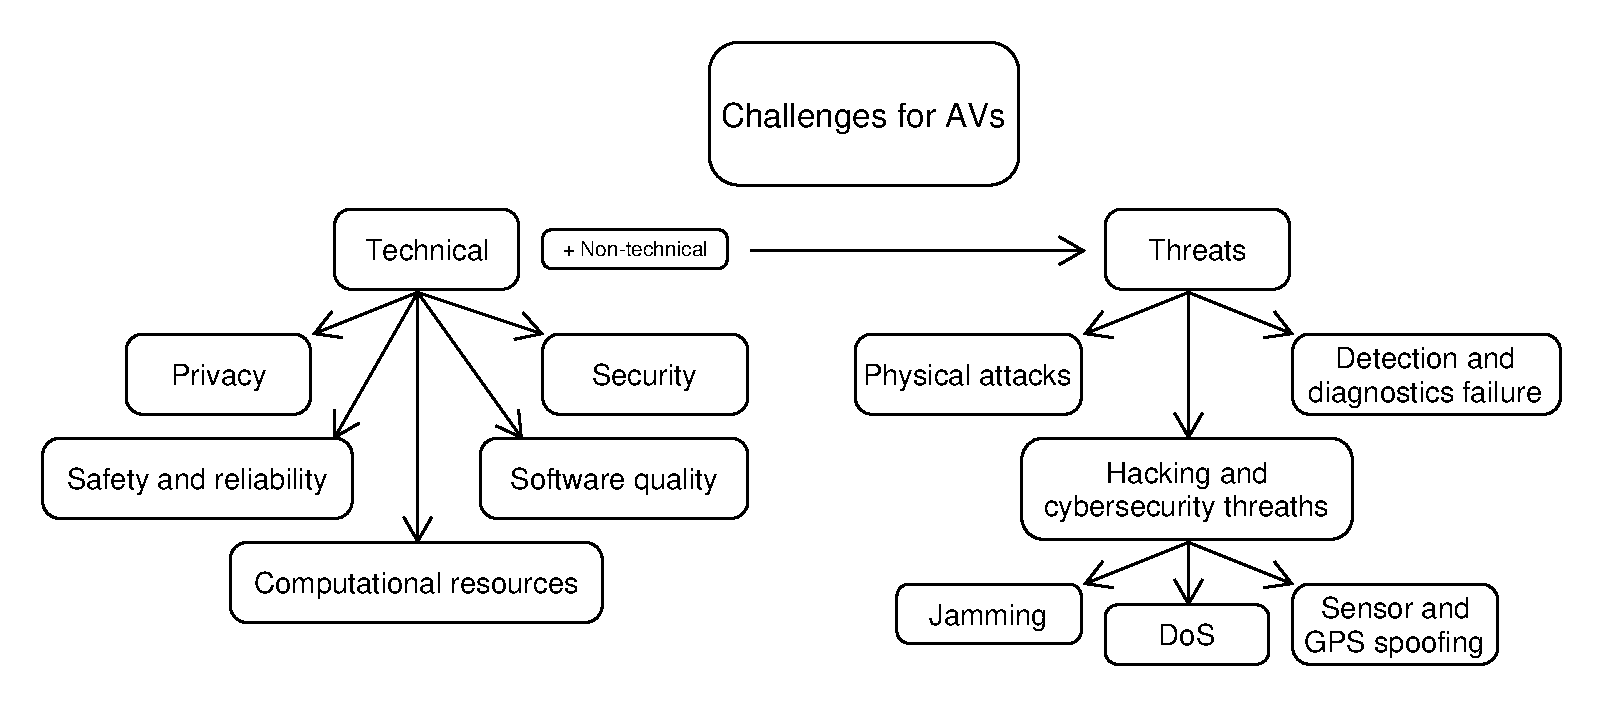
\includegraphics[width=10.4cm]{challenges.pdf}

    \end{figure}
\end{frame}

%------------------------------------------------------------------------------------------------------------------------------

\section{Future directions}

\begin{frame}[fragile=singleslide]\frametitle{\bf{Future directions}}
\begin{itemize}

\item {\textbf{Efficiency}}
         \begin{itemize}
	\item AI enhancements
	\item Edge computing integration
         \item Advanced sensor fusion
	\end{itemize}
\item {\textbf{Connection}}
         \begin{itemize}
	\item V2X communication enhancements
         \item 5G connectivity
	\end{itemize}
\item {\textbf{Security}}
         \begin{itemize}
	\item Cybersecurity measures
         \item Continuous monitoring
	\end{itemize}
\item {\textbf{Safety}}
         \begin{itemize}
	\item Human behavior prediction
         \item Advanced Driver Assistance Systems (ADAS) 
         \item Predictive analytics
	\end{itemize}
\end{itemize}

\end{frame}

%------------------------------------------------------------------------------------------------------------------------------
\section*{Conclusion}

\begin{frame}[fragile=singleslide]\frametitle{\bf{Conclusion}}
    \centering
    \begin{figure}
        \centering
        \caption{Levels of automation\footnote{\tiny{\url{https://www.statista.com/chart/25754/newly-registered-cars-by-autonomous-driving-level/}}}}
        \vspace*{-1.1cm}
        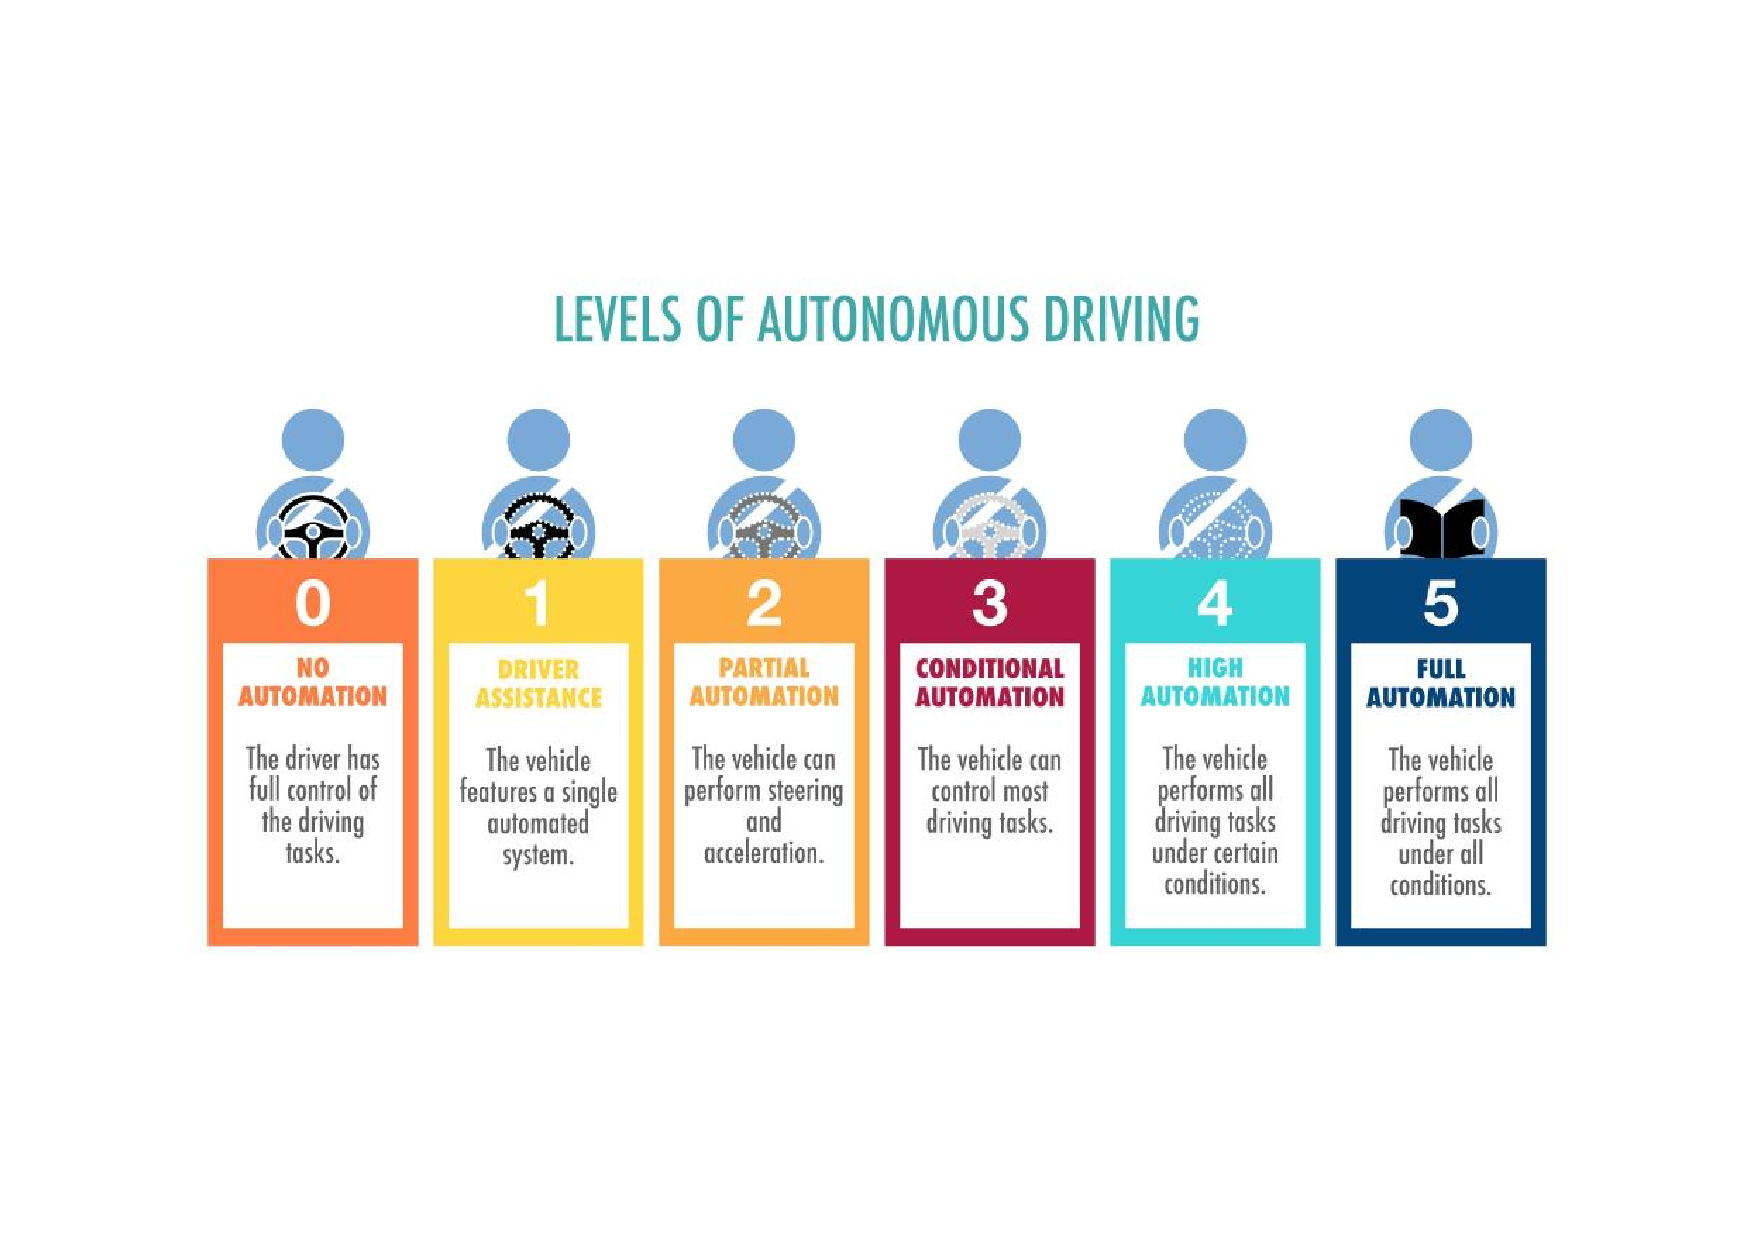
\includegraphics[width=10cm]{levels.pdf}
    \end{figure}
\end{frame}


%------------------------------------------------------------------------------------------------------------------------------

\begin{frame}[fragile=singleslide]
\centering
\hspace*{1cm}
\vspace*{-1cm}
\LARGE{\textbf{Thank you for your attention}}
\end{frame}


\end{document}


